\documentclass[11pt]{article}

% --- Encodage et langue ---
\usepackage[french]{babel}
\usepackage[utf8]{inputenc}
\usepackage[T1]{fontenc}
\usepackage{lmodern}

% --- Packages scientifiques et graphiques ---
\usepackage{amsmath,amssymb}
\usepackage{graphicx}
\usepackage{booktabs}
\usepackage[margin=2.5cm]{geometry}
\usepackage{hyperref}
\usepackage{float}
\usepackage{caption}
\usepackage{subcaption}
\usepackage{tikz}
\usepackage{xcolor}
\usepackage{listings}
\usetikzlibrary{positioning,arrows.meta,calc,shadows,shapes.geometric}

\graphicspath{{figures/}{assets/}}
\linespread{1.08}
\hypersetup{
  colorlinks=true,
  linkcolor=black,
  citecolor=black,
  urlcolor=blue
}

% --- Configuration de l'affichage du code GAML ---
\lstdefinelanguage{GAML}{
  morekeywords={
    model,global,species,experiment,init,reflex,action,aspect,output,display,chart,
    data,monitor,parameter,create,ask,do,if,else,loop,over,where,when,return,returns,
    match,switch,default,true,false,nil,map,list,int,float,string,bool,point,geometry,rgb
  },
  sensitive=true,
  morecomment=[l]{//},
  morecomment=[s]{/*}{*/},
  morestring=[b]"
}

\lstset{
  language=GAML,
  basicstyle=\ttfamily\scriptsize,
  keywordstyle=\color{blue!70!black}\bfseries,
  commentstyle=\color{gray!70!black},
  stringstyle=\color{green!40!black},
  numbers=left,
  numberstyle=\tiny\color{gray},
  stepnumber=1,
  numbersep=6pt,
  breaklines=true,
  breakatwhitespace=false,
  showstringspaces=false,
  keepspaces=true,
  frame=single,
  columns=fullflexible,
  inputencoding=utf8,
  extendedchars=true,
  literate=
    {é}{{\'e}}1 {è}{{\`e}}1 {ê}{{\^e}}1 {ë}{{\"e}}1
    {à}{{\`a}}1 {â}{{\^a}}1
    {ù}{{\`u}}1 {û}{{\^u}}1
    {î}{{\^i}}1 {ï}{{\"i}}1
    {ô}{{\^o}}1
    {ç}{{\c{c}}}1
    {É}{{\'E}}1 {È}{{\`E}}1 {À}{{\`A}}1 {Ç}{{\c{C}}}1
    {œ}{{\oe}}1
    {×}{{$\times$}}1
    {—}{{--}}1 {–}{{--}}1
}

\begin{document}

% ---------------- Page de garde ----------------
\thispagestyle{empty}
\begin{center}
  {\bfseries\small RÉPUBLIQUE DÉMOCRATIQUE DU CONGO} \\[2pt]
  {\bfseries\small UNIVERSITÉ DE KINSHASA} \\[6pt]
  
\includegraphics[width=0.14\textwidth]{images.png} \\[6pt]
  {\small FACULTÉ DES SCIENCES ET TECHNOLOGIES \\ Mention Mathématiques, Statistique et Informatique} \\[2pt]
  {\small B.P. 190 KINSHASA XI} \\[6pt]
  {\small Master 1} \\[6pt]
  {\bfseries\large TRAVAIL PRATIQUE DE SYSTÈME MULTI-AGENT} \\[10pt]
  {\Large\bfseries Modélisation et simulation d'une station de recharge \\ pour véhicules électriques} \\[14pt]
  {\normalsize Projet 8 : Station de Recharge pour Véhicules Électriques} \\[14pt]
  {\normalsize DUASENGE MAYANO Brummel} \\
  {\normalsize MAKWIZA MBALA Judicael} \\
  {\normalsize MFUSHI KAPALAY Stéphane}\\ [10pt]
  \textbf{Professeur }{\normalsize KASEREKA Selain} \\
  \textbf{Doctorant }{\normalsize MBAYANDJAMBE Alidor} \\[6pt]
  {\normalsize Mai 2026}
\end{center}

\vspace{8pt}

\begin{abstract}
Ce travail présente une modélisation multi-agent du fonctionnement d'une station de recharge pour véhicules électriques soumise à une demande aléatoire et à des ressources limitées. Le modèle retenu est un modèle à états discrets couplé à une file d'attente multi-serveurs hétérogène : les véhicules sont des agents capables d'arriver, d'attendre, de se connecter à une borne, d'être servis ou d'abandonner, tandis que les bornes alternent entre disponibilité, occupation, panne et maintenance. La simulation intègre des arrivées fluctuantes avec pic en soirée, des arrivées groupées, des pannes de bornes et une variation de la puissance délivrée liée au réseau. Les indicateurs étudiés sont le taux d'occupation moyen des bornes, la longueur moyenne de la file, le temps d'attente moyen, le taux d'abandon et le taux de satisfaction global. Le modèle est implémenté en GAML sur GAMA Platform, avec une configuration de 10 bornes lentes, 8 bornes accélérées et 5 bornes rapides.
\end{abstract}
\newpage
\section{Introduction}
Ce travail analyse la dynamique de la simulation du fonctionnement en temps réel d'une station de recharge pour véhicules électriques. Le problème étudié est celui d'un service soumis simultanément à une demande variable et à une capacité limitée : les véhicules n'arrivent pas de manière régulière, les bornes peuvent être occupées ou indisponibles, et les usagers ne tolèrent pas tous la même durée d'attente. Le sujet impose donc de représenter à la fois des ressources techniques, des comportements individuels et des indicateurs globaux de performance.

Une approche multi-agent est adaptée à ce type de système, car elle permet de représenter chaque entité active par ses états, ses décisions et ses interactions. Dans le cadre du cours de systèmes multi-agents, un agent est considéré comme une entité située dans un environnement, capable de percevoir certaines informations et d'agir de manière autonome. La station de recharge constitue ici un environnement dynamique et non déterministe : de nouveaux véhicules peuvent arriver, les bornes changent d'état, la puissance disponible varie, et les décisions locales produisent des effets collectifs visibles sur la file d'attente et la satisfaction.

Les modèles de files d'attente sont utilisés pour dimensionner les stations et estimer la qualité de service, tandis que les modèles stochastiques à arrivées variables permettent de représenter un flux entrant dépendant du temps~\cite{kim2017}. Les simulations agent-based sont également employées pour étudier les temps d'attente, les politiques de coordination et l'utilisation des chargeurs~\cite{garcia2018,karlsson2023}. Notre modèle combine ces idées à l'échelle d'une station : agents individuels, états discrets, file d'attente et indicateurs de performance.

L'objectif de ce travail est triple. Premièrement, il s'agit de proposer un modèle multi-agent à états discrets décrivant les véhicules, les bornes et la file d'attente. Deuxièmement, il faut formaliser les principales équations de fonctionnement déduites du code GAML : arrivée des véhicules, durée de recharge, attente, abandon, occupation et satisfaction. Troisièmement, le modèle doit être simulé dans GAMA Platform afin d'analyser les sorties graphiques produites par l'expérience.

Le rapport est organisé de la manière suivante. La section~\ref{sec:cadre} présente brièvement le cadre SMA et GAMA utilisé. La section~\ref{sec:modele} décrit le modèle des véhicules, des bornes et de la file. La section~\ref{sec:formulation} donne la formulation mathématique issue du code. La section~\ref{sec:parametres} précise les paramètres de simulation. La section~\ref{sec:implementation} résume l'implémentation GAML. La section~\ref{sec:resultats} présente les résultats obtenus et leur interprétation. Enfin, la conclusion synthétise les apports et limites du modèle.
\newpage
\section{Cadre SMA et GAMA}\label{sec:cadre}

Le système étudié est composé de plusieurs agents qui interagissent autour d'une ressource limitée. Les véhicules sont des agents dynamiques : ils arrivent dans la station, évaluent la disponibilité des bornes, rejoignent éventuellement une file et peuvent abandonner si l'attente devient incompatible avec leur tolérance ou leur urgence. Les bornes sont des agents techniques : elles peuvent être libres, occupées, en panne ou en maintenance. La station joue le rôle d'agent de coordination, car elle conserve la file d'attente et attribue les bornes libres selon une politique de service.

Le modèle est réactif : les comportements sont principalement décrits par des règles exécutées à chaque pas de temps. Dans GAML, ces comportements sont codés par des \texttt{reflex}. La structure du modèle respecte le paradigme standard de GAMA, séparant la définition des espèces \texttt{(species)}, les comportements \texttt{(reflex)} et l'expérimentation \texttt{(experiment)}.



GAMA Platform est retenue comme environnement de simulation, car elle fournit un langage de modélisation multi-agent, GAML, et des sorties graphiques directement exploitables, notamment les séries temporelles, histogrammes et diagrammes circulaires. Ces sorties sont utiles pour analyser simultanément les comportements microscopiques et les indicateurs macroscopiques du système.

\section{Description du modèle}\label{sec:modele}

\subsection{États des véhicules}

Les véhicules ne sont pas modélisés comme une population continue, mais comme des agents individuels. Chaque véhicule possède un état discret. Un véhicule nouvellement créé est dans l'état \texttt{arriving}. S'il trouve une borne libre, il passe directement à l'état \texttt{charging}. Si aucune borne n'est libre, il rejoint l'état \texttt{waiting}. Pendant l'attente, il réévalue sa situation : d'une décision autonome basée sur son état interne (mémorisation de son temps d'attente) si l'attente estimée dépasse sa tolérance, ou si son urgence est élevée après une attente prolongée, il passe à l'état \texttt{abandoned}. Lorsqu'une recharge se termine, le véhicule passe à l'état \texttt{served}, puis disparaît du modèle après comptabilisation des indicateurs.

\subsection{États des bornes}

Les bornes suivent quatre états. Une borne \texttt{libre} peut recevoir un véhicule et devenir \texttt{occupée}. Pendant la recharge, elle reste occupée jusqu'à ce que le véhicule atteigne son objectif de batterie ou que le temps de recharge restant devienne nul. Une borne libre ou occupée peut tomber en \texttt{panne} selon une probabilité par pas de temps. Si la panne survient pendant une recharge, le véhicule branché est replacé en tête de file. Après la durée de panne, la borne passe brièvement en \texttt{maintenance}, puis redevient disponible.

\begin{figure}[H]
\centering
\resizebox{\textwidth}{!}{%
\begin{tikzpicture}[
  >=Stealth,
  comp/.style={draw=black, thick, rounded corners, minimum width=3.0cm, minimum height=1.0cm, align=center, font=\bfseries, text=white},
  borne/.style={draw=black, thick, rounded corners, minimum width=2.7cm, minimum height=1.0cm, align=center, font=\bfseries},
  arr/.style={->, thick, shorten >=2pt, shorten <=2pt},
  lab/.style={font=\small, align=center}
]
  % Vehicules
  \node[comp, fill=blue!70!black] (A) at (0,2.5) {Arriving};
  \node[comp, fill=yellow!55!black] (W) at (6,2.5) {Waiting};
  \node[comp, fill=cyan!60!black] (C) at (12,2.5) {Charging};
  \node[comp, fill=green!55!black] (S) at (18,2.5) {Served};
  \node[comp, fill=red!70!black] (D) at (1,0.6) {Abandoned};

  \draw[arr] (A) -- node[above,lab] {aucune borne libre} (W);
  \draw[arr] (A) to[bend left=18] node[above,lab] {borne libre} (C);
  \draw[arr] (W) -- node[above,lab] {attribution} (C);
  \draw[arr] (C) -- node[above,lab] {recharge terminée} (S);
  \draw[arr] (W) -- node[right,lab] {tolérance dépassée\\ou urgence élevée} (D);
  \draw[arr] (C) to[bend left=35] node[below,lab] {panne de borne\\retour en file} (W);

  % Bornes
  \node[borne, fill=green!25] (BL) at (0,-3.1) {Libre};
  \node[borne, fill=orange!35] (BO) at (6,-3.1) {Occupée};
  \node[borne, fill=red!30] (BP) at (12,-3.1) {Panne};
  \node[borne, fill=gray!30] (BM) at (18,-3.1) {Maintenance};

  \draw[arr] (BL) -- node[above,lab] {connexion} (BO);
  \draw[arr] (BO) to[bend left=18] node[below,lab] {fin recharge} (BL);
  \draw[arr] (BL) to[bend left=18] node[above,lab] {panne} (BP);
  \draw[arr] (BO) -- node[above,lab] {panne} (BP);
  \draw[arr] (BP) -- node[above,lab] {réparation} (BM);
  \draw[arr] (BM) to[bend left=22] node[below,lab] {retour service} (BL);
\end{tikzpicture}
}
\caption{Diagramme d'états des véhicules et des bornes de recharge.}
\label{fig:modele-etats}
\end{figure}

La Figure~\ref{fig:modele-etats} synthétise l'organisation du système. Les états du haut décrivent le parcours d'un véhicule dans la station, tandis que ceux du bas décrivent la disponibilité opérationnelle des bornes. Cette séparation permet de suivre à la fois la demande et l'état de l'offre de recharge.

\subsection{File d'attente et serveurs de recharge}

La station est modélisée comme une file d'attente multi-serveurs : les clients sont les véhicules et les serveurs sont les bornes. Elle est hétérogène parce que les serveurs n'ont pas tous la même puissance : les bornes lentes, accélérées et rapides ne produisent pas la même durée de recharge. Le code utilise par défaut une file unique et une politique FIFO, tout en prévoyant d'autres politiques de sélection : plus faible batterie, plus forte urgence ou respect de la préférence de puissance.

Ce formalisme est plus adapté qu'un système d'équations différentielles ordinaires, car l'ordre dans la file, la disponibilité instantanée des bornes, les pannes et les décisions d'abandon sont des événements discrets. Les équations du rapport décrivent donc les règles de calcul et les indicateurs du système plutôt qu'une dynamique continue de populations.
\newpage
\section{Formulation mathématique}\label{sec:formulation}

Le modèle n'est pas formulé comme un système d'équations différentielles continu. Il s'agit d'une simulation à pas discret, avec un pas de temps de $\Delta t = 1$ minute. Les équations suivantes décrivent les calculs effectués par le code GAML à chaque cycle. Elles traduisent les mécanismes de la file d'attente et des agents : arrivée, recharge, attente, abandon et indicateurs.

\subsection{Arrivée fluctuante des véhicules}

Le taux instantané d'arrivée dépend de l'heure simulée $h(t)$ et augmente autour de 19 h. Le code utilise la forme :
\[
\lambda(t) = \lambda_0 \left(1 + a \exp\left[-\frac{(h(t)-19)^2}{2\sigma^2}\right]\right),
\]
où $\lambda_0$ est le taux de base, $a$ l'amplitude de variation et $\sigma$ la largeur du pic. À chaque pas de temps, un véhicule peut être créé avec la probabilité :
\[
p_{\mathrm{arr}}(t)=\min\left(1,\lambda(t)\frac{\Delta t}{1\ \mathrm{h}}\right).
\]
Le modèle ajoute aussi des arrivées groupées : avec une probabilité $p_{\mathrm{burst}}$, un groupe de véhicules supplémentaires est créé.

\subsection{Énergie et durée de recharge}

Pour un véhicule $v$, le déficit de batterie à combler est :
\[
\Delta b_v = b_v^{\mathrm{cible}} - b_v,
\]
où $b_v$ est le niveau courant de batterie et $b_v^{\mathrm{cible}}$ l'objectif de recharge. L'énergie à fournir est :
\[
E_v = \frac{\Delta b_v}{100} C_v,
\]
avec $C_v$ la capacité de batterie du véhicule en kWh. La puissance réellement délivrée par une borne $i$ est :
\[
P_i^{\mathrm{eff}} = P_i f_{\mathrm{res}},
\]
où $P_i$ est la puissance nominale de la borne et $f_{\mathrm{res}}\in[0.5,1]$ représente la contrainte du réseau. La durée de recharge initialement estimée est donc :
\[
T_v = \frac{E_v}{P_i^{\mathrm{eff}}}.
\]

\subsection{Mise à jour de la batterie}

À chaque pas, l'énergie fournie au véhicule branché est :
\[
\Delta E_v = P_i^{\mathrm{eff}}\frac{\Delta t}{1\ \mathrm{h}}.
\]
Le niveau de batterie est mis à jour par :
\[
b_v(t+\Delta t)=\min\left(100,\ b_v(t)+100\frac{\Delta E_v}{C_v}\right).
\]
La recharge s'arrête lorsque le véhicule atteint sa batterie cible ou lorsque le temps de recharge restant devient nul.

\subsection{Estimation de l'attente et indicateurs}

Lorsque l'affichage du temps d'attente est activé, la station estime l'attente d'un véhicule en file à partir de la taille de la file $Q(t)$, du nombre de bornes actives $B_{\mathrm{act}}(t)$ et d'un temps moyen simplifié de recharge de 30 minutes :
\[
\widehat{W}(t)=\frac{Q(t)}{B_{\mathrm{act}}(t)}\times 30\ \mathrm{minutes}.
\]
Un véhicule peut abandonner si cette estimation dépasse sa tolérance ou si son temps d'attente effectif devient trop long.

Les indicateurs globaux utilisés dans le rapport sont :
\[
\tau_{\mathrm{occ}}(t)=\frac{B_{\mathrm{occ}}(t)}{B_{\mathrm{total}}},
\qquad
\overline{\tau}_{\mathrm{occ}}=\frac{1}{n}\sum_{k=1}^{n}\tau_{\mathrm{occ}}(k),
\]
\[
\overline{Q}=\frac{1}{n}\sum_{k=1}^{n}Q(k),
\qquad
T_{\mathrm{abandon}}=\frac{N_{\mathrm{abandons}}}{N_{\mathrm{arrivees}}},
\]
et, pour un véhicule servi,
\[
S_v=\max\left(0,1-\frac{W_v}{W_v^{\max}}\right)\times \beta_v,
\]
où $W_v$ est le temps d'attente observé, $W_v^{\max}$ la tolérance du véhicule, et $\beta_v$ vaut $1$ si la préférence de puissance est respectée, sinon $0.7$ dans le code.
\newpage
\section{Paramètres du modèle}\label{sec:parametres}

Les paramètres retenus correspondent au code GAML mis à jour pour ce rapport. Les bornes sont réparties en trois catégories de puissance afin de représenter une station hétérogène.

\begin{table}[H]
\centering
\caption{Paramètres principaux de la simulation.}
\label{tab:parametres}
\begin{tabular}{@{}lll@{}}
\toprule
Catégorie & Paramètre & Valeur \\
\midrule
Bornes & Nombre de bornes lentes & 10 \\
Bornes & Nombre de bornes accélérées & 8 \\
Bornes & Nombre de bornes rapides & 5 \\
Puissance & Borne lente & 7 kW \\
Puissance & Borne accélérée & 22 kW \\
Puissance & Borne rapide & 50 kW \\
Temps & Pas de simulation & 1 minute \\
Arrivées & Taux de base & 0.5 véhicule/heure \\
Arrivées & Amplitude du pic & 1.5 \\
Arrivées & Largeur du pic & 3 h \\
Stochastique & Probabilité de panne par pas & 0.0005 \\
Stochastique & Probabilité d'arrivée groupée & 0.02 \\
Stochastique & Taille d'un groupe & 4 véhicules \\
File & Politique par défaut & FIFO \\
File & Organisation par défaut & File unique \\
Information & Affichage du temps d'attente & Activé \\
\bottomrule
\end{tabular}
\end{table}

Chaque véhicule est créé avec un niveau de batterie initial tiré entre 5\% et 40\%, une batterie cible de 80\%, une capacité comprise entre 30 et 80 kWh, une urgence tirée entre 0 et 1, une tolérance d'attente comprise entre 15 et 90 minutes, et une préférence de puissance choisie parmi les trois types de bornes.
\newpage
\section{Implémentation dans GAMA}\label{sec:implementation}

L'implémentation est structurée autour de trois espèces. L'espèce \texttt{station} centralise les bornes, les files et l'attribution des ressources. Elle contient les actions d'enfilement, de retrait, de remise en file après panne et de sélection du prochain véhicule. La sélection peut suivre plusieurs politiques prévues dans le code : FIFO, plus faible batterie, plus forte urgence ou préférence de puissance.

L'espèce \texttt{borne} représente les points de recharge. Elle calcule la durée de recharge à partir de l'énergie demandée et de la puissance effective, met à jour la batterie du véhicule branché, libère la borne à la fin du service et gère les pannes. Lorsqu'une panne touche une borne occupée, le véhicule concerné est replacé dans la file.

L'espèce \texttt{vehicule} représente la demande. À la création, le véhicule tente d'abord une connexion directe. S'il ne trouve pas de borne disponible, il attend. Pendant l'attente, il actualise son temps d'attente, consulte l'estimation si l'information est activée et peut abandonner. Lorsqu'il est servi, il contribue au calcul du temps d'attente moyen, de la satisfaction et du nombre total de véhicules servis.

L'expérience \texttt{Station\_Recharge} expose les paramètres de bornes, de puissance, de file, d'information et d'événements stochastiques. Les sorties GAMA comprennent une carte de la station, quatre séries temporelles, deux graphiques de répartition et un histogramme des indicateurs globaux.

\section{Résultats de simulation et interprétation}\label{sec:resultats}

Les figures ci-dessous illustrent l'état de l'expérience au cycle 969. L'interprétation se base aux sorties observées et aux mécanismes codés.

\begin{figure}[H]
\centering
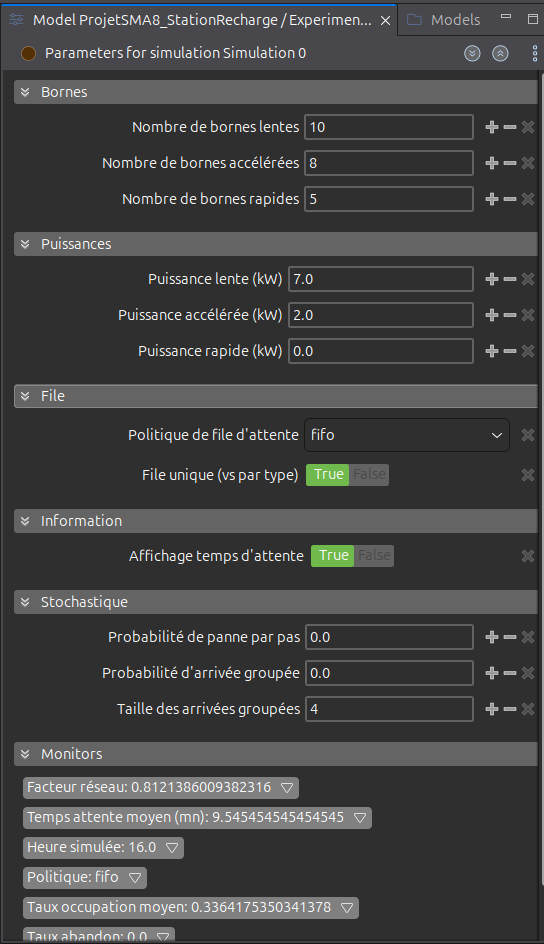
\includegraphics[width=0.34\textwidth]{ProjetSMA8_StationRecharge_paramettre_de_lancement_a_signaler_dans_le_rapport.png}
\caption{Paramètres de lancement affichés dans l'interface GAMA.}
\label{fig:parametres-lancement}
\end{figure}

La Figure~\ref{fig:parametres-lancement} documente les paramètres utilisés au lancement de l'expérience. Cette capture est importante pour relier les résultats aux conditions de simulation : nombre de bornes, puissances, politique de file, affichage d'information et paramètres stochastiques. Le dimensionnement retenu pour la simulation de référence s'appuie sur la capacité totale de la station à 23 bornes.


\begin{figure}[H]
\centering
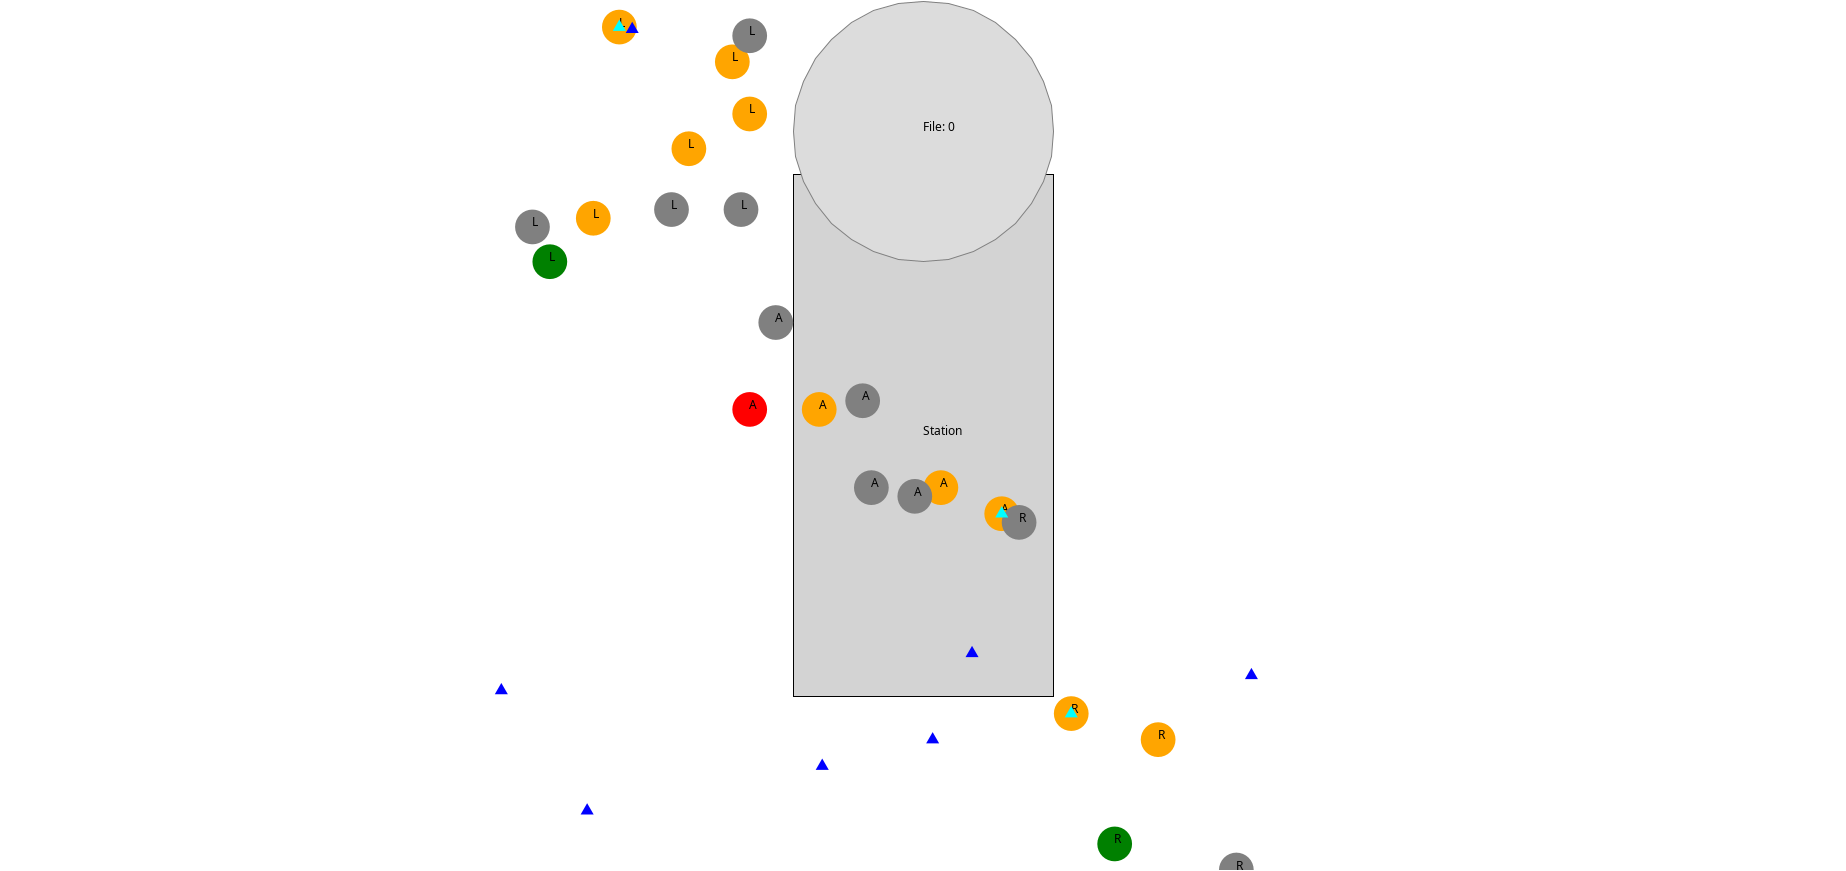
\includegraphics[width=0.95\textwidth]{ProjetSMA8_StationRecharge_model_display_CarteStation_cycle_969_time_1778225754810.png}
\caption{Carte de la station au cycle 969. Les bornes et véhicules sont affichés dans l'environnement de simulation.}
\label{fig:carte-station}
\end{figure}

La Figure~\ref{fig:carte-station} donne une vue spatiale synthétique de la station. Les bornes sont distribuées dans l'espace et changent de couleur selon leur état opérationnel. Les véhicules en attente sont regroupés dans la zone de file, tandis que les véhicules en recharge sont associés à une borne. Cette visualisation confirme que le modèle relie les états internes des agents à une représentation spatiale lisible.

\begin{figure}[H]
\centering
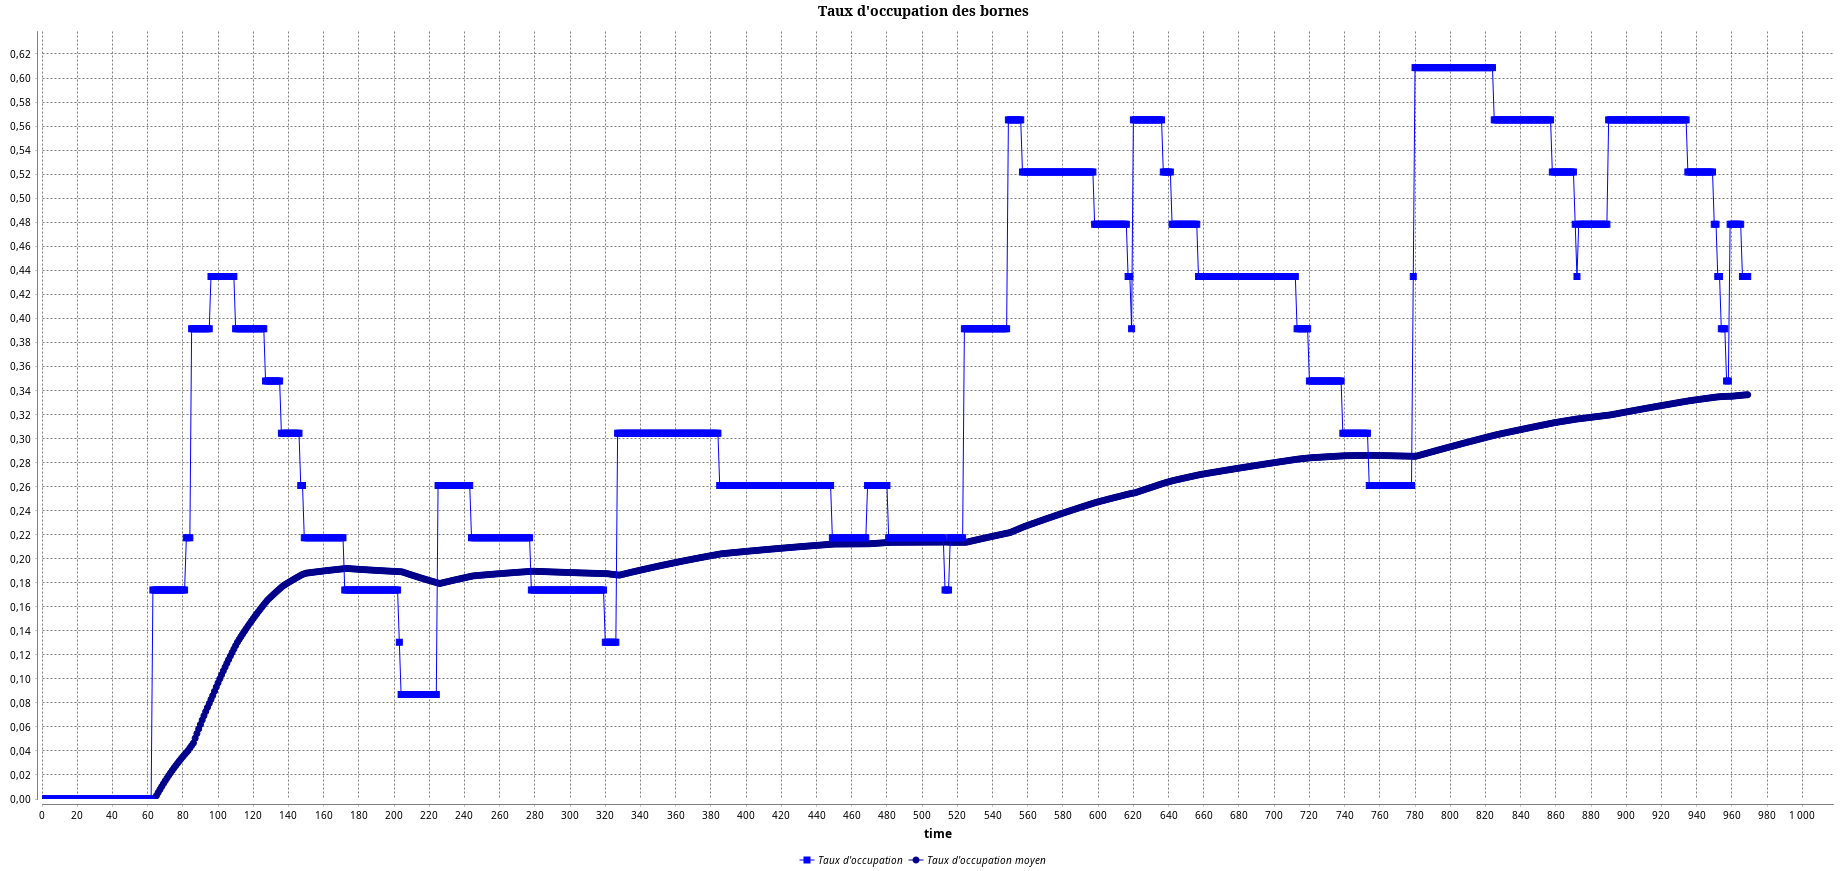
\includegraphics[width=0.95\textwidth]{ProjetSMA8_StationRecharge_model_display_Occupation_Series_cycle_969_time_1778225872696.png}
\caption{Évolution du taux d'occupation instantané et du taux d'occupation moyen des bornes.}
\label{fig:occupation}
\end{figure}

La Figure~\ref{fig:occupation} suit la proportion de bornes occupées au cours du temps. Le taux instantané varie avec les arrivées, la durée de recharge, les libérations de bornes et les pannes éventuelles. La courbe moyenne amortit ces variations et fournit une mesure plus stable de l'utilisation globale de la station. Un taux d'occupation durablement élevé signale une forte pression sur les ressources, tandis qu'un taux faible indique une capacité disponible.

\begin{figure}[H]
\centering
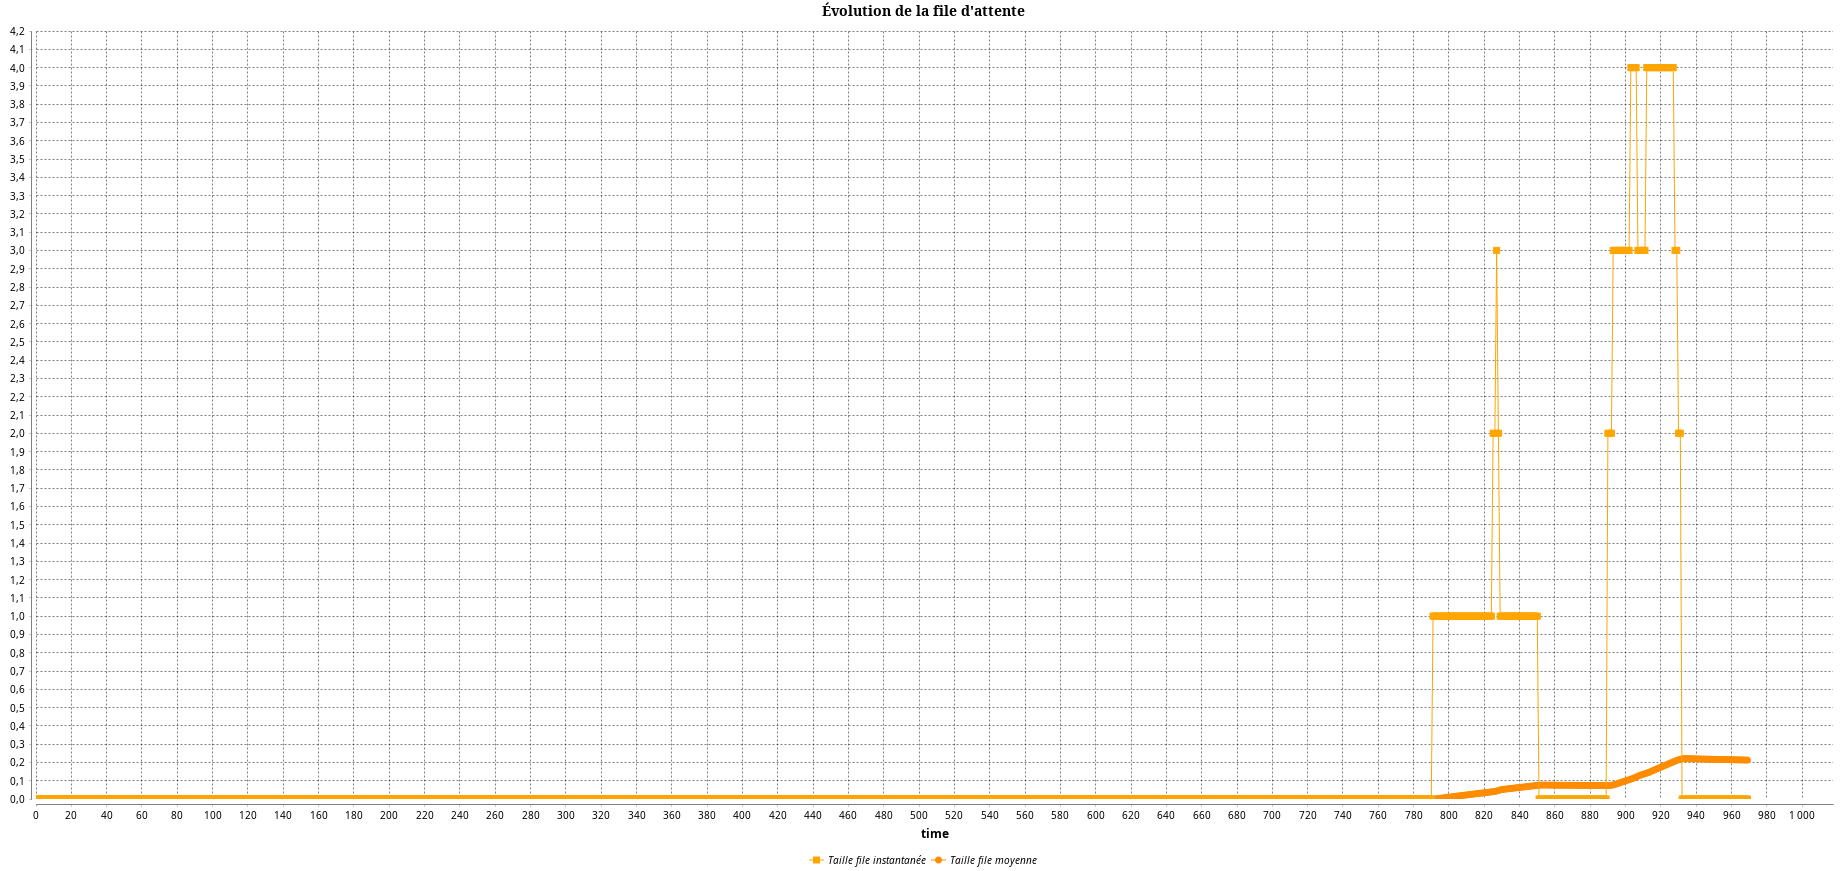
\includegraphics[width=0.95\textwidth]{ProjetSMA8_StationRecharge_model_display_File_Series_cycle_969_time_1778225987395.png}
\caption{Évolution de la taille instantanée et moyenne de la file d'attente.}
\label{fig:file}
\end{figure}

La Figure~\ref{fig:file} montre la dynamique de congestion. La file augmente lorsque le flux d'arrivée dépasse momentanément la capacité de service, notamment lors des arrivées groupées ou lorsque plusieurs bornes sont indisponibles. Elle diminue lorsque des bornes se libèrent et que la station attribue des véhicules en attente. La comparaison entre la taille instantanée et la moyenne permet de distinguer les pics ponctuels d'une congestion persistante.

\begin{figure}[H]
\centering
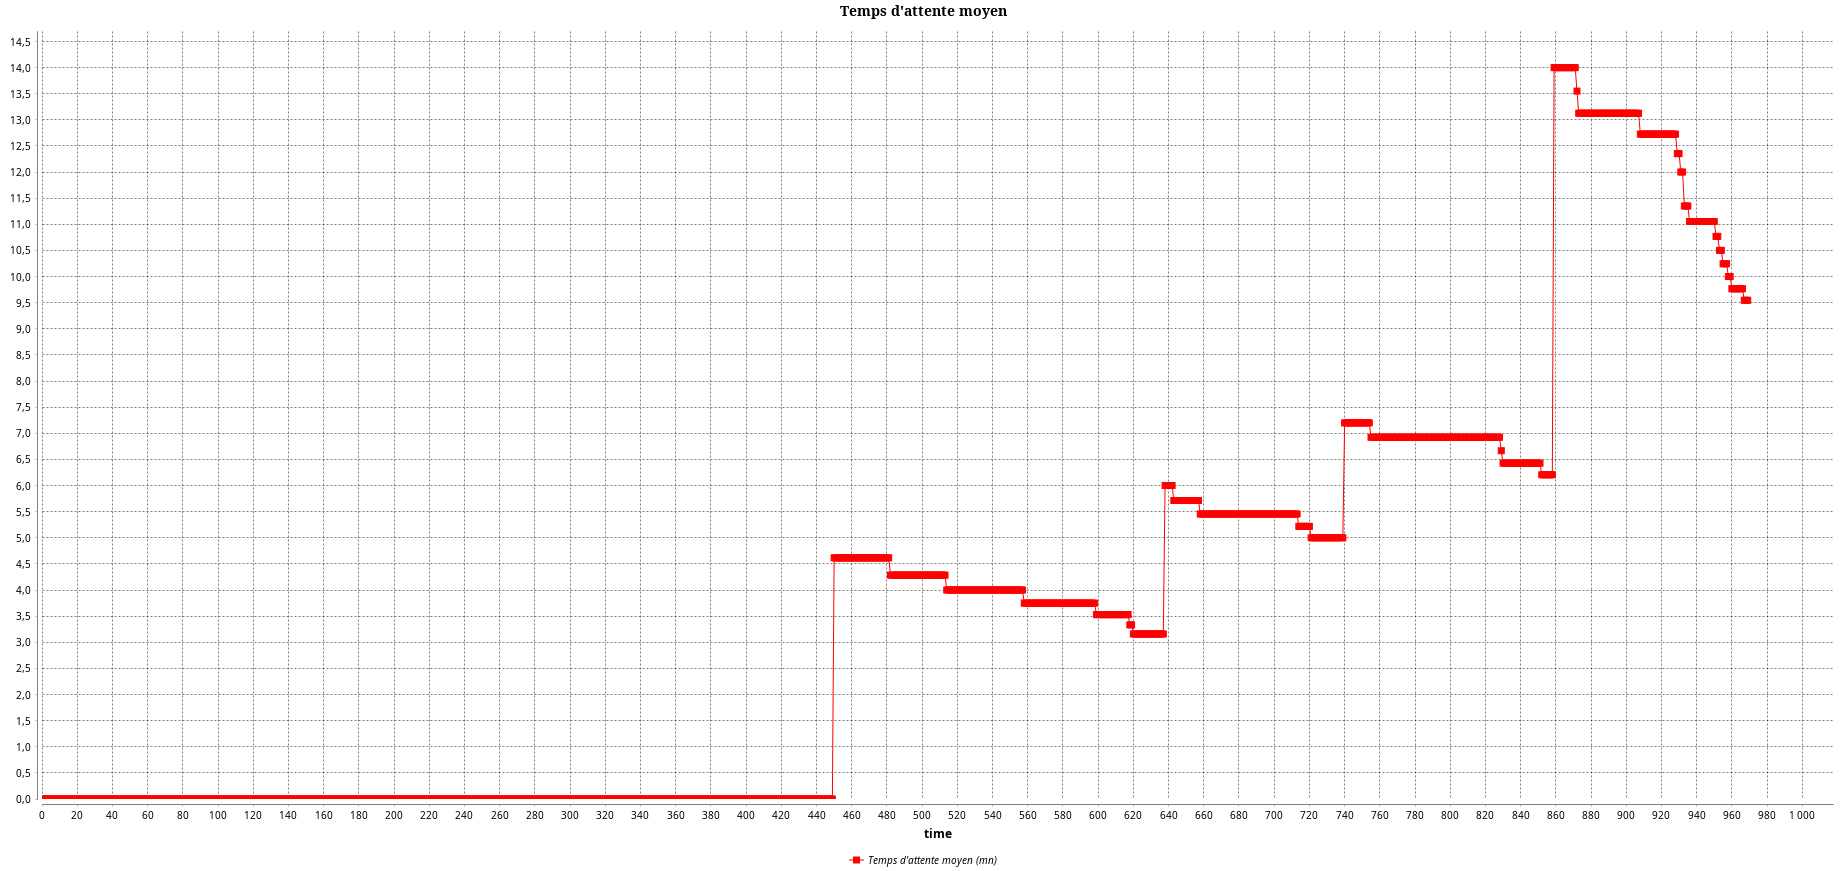
\includegraphics[width=0.95\textwidth]{ProjetSMA8_StationRecharge_model_display_Attente_Series_cycle_969_time_1778226051399.png}
\caption{Évolution du temps d'attente moyen des véhicules servis.}
\label{fig:attente}
\end{figure}

La Figure~\ref{fig:attente} présente le temps d'attente moyen calculé à partir des véhicules effectivement servis. Cet indicateur est directement lié à la satisfaction : plus l'attente se rapproche de la tolérance individuelle, plus la satisfaction diminue. Il complète la taille de file, car une file courte peut encore produire une attente importante si les recharges en cours sont longues ou si la puissance effective du réseau est réduite.

\begin{figure}[H]
\centering
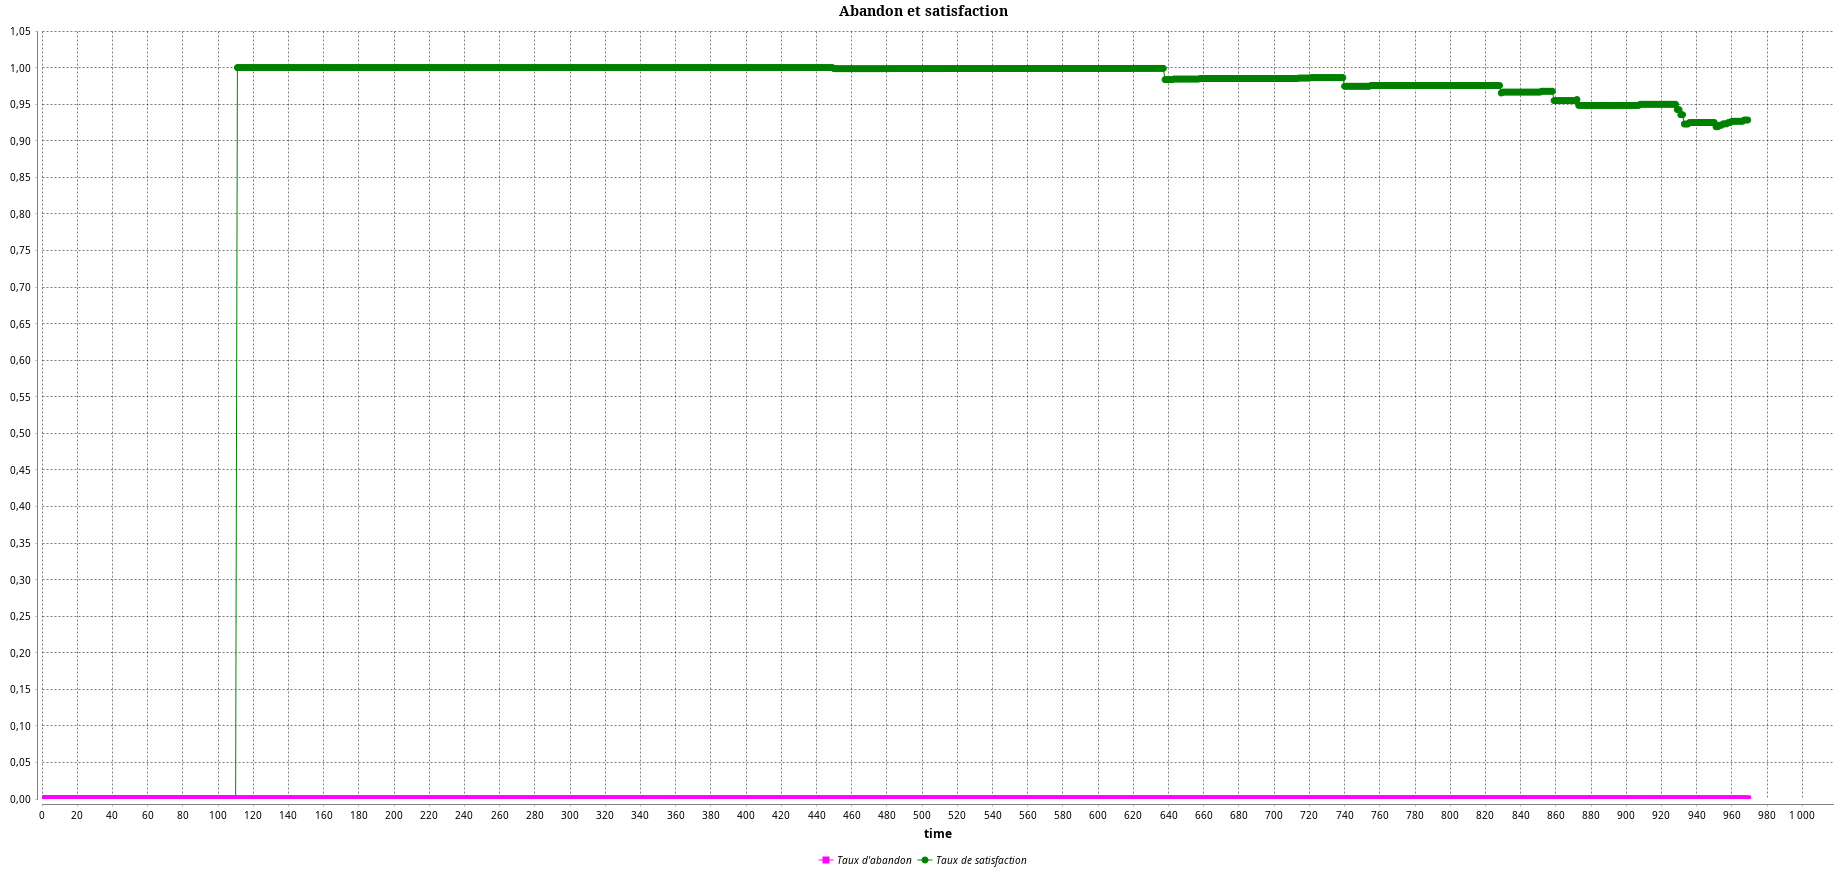
\includegraphics[width=0.95\textwidth]{ProjetSMA8_StationRecharge_model_display_Abandon_Satisfaction_cycle_969_time_1778225899254.png}
\caption{Évolution conjointe du taux d'abandon et du taux de satisfaction.}
\label{fig:abandon-satisfaction}
\end{figure}

La Figure~\ref{fig:abandon-satisfaction} met en relation deux indicateurs complémentaires. Le taux d'abandon mesure la part des véhicules partis sans recharge, tandis que la satisfaction agrège l'effet de l'attente et du respect de la préférence de puissance. Une hausse des abandons traduit une dégradation de l'accessibilité du service. Une satisfaction élevée indique au contraire que les véhicules servis l'ont été avec une attente compatible avec leur tolérance et, autant que possible, avec leur préférence de recharge.

\begin{figure}[H]
\centering
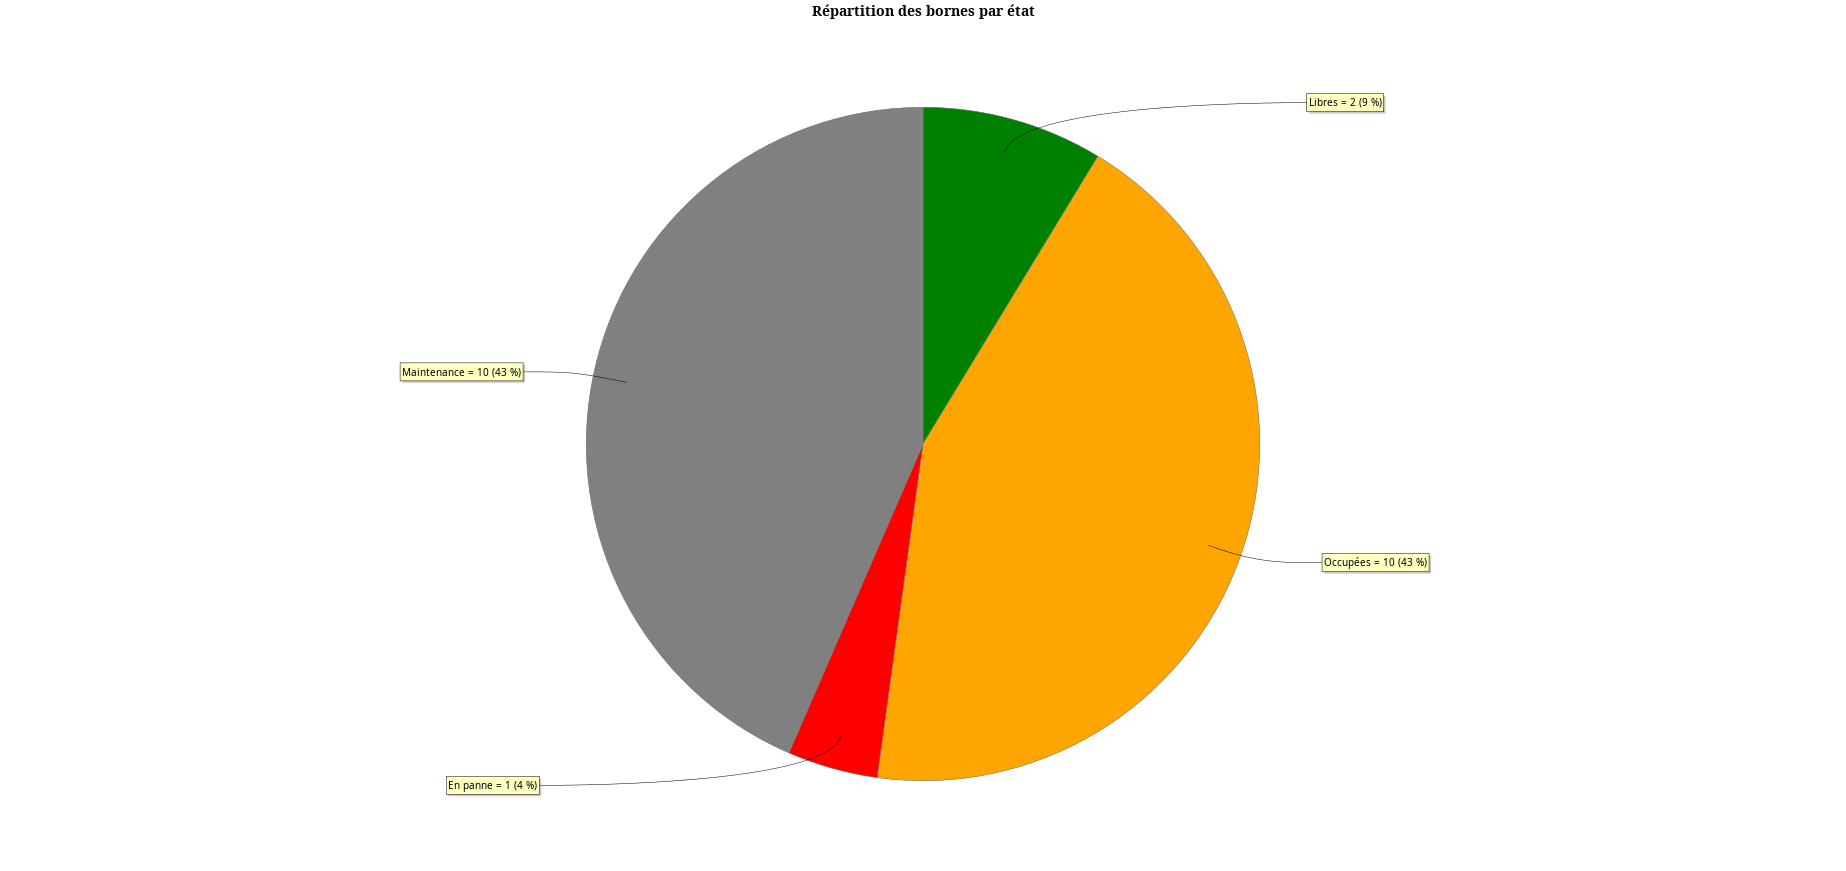
\includegraphics[width=0.95\textwidth]{ProjetSMA8_StationRecharge_model_display_Repartition_Bornes_Pie_cycle_969_time_1778225957741.png}
\caption{Répartition des bornes selon leur état : libres, occupées, en panne ou en maintenance.}
\label{fig:repartition-bornes}
\end{figure}

La Figure~\ref{fig:repartition-bornes} décrit l'état opérationnel de l'offre de recharge à l'instant observé. La part des bornes libres représente la capacité immédiatement disponible. La part occupée correspond à la charge de service en cours. Les états panne et maintenance réduisent temporairement la capacité effective, ce qui peut augmenter la file et le temps d'attente même si le nombre total de bornes installé est important.

\begin{figure}[H]
\centering
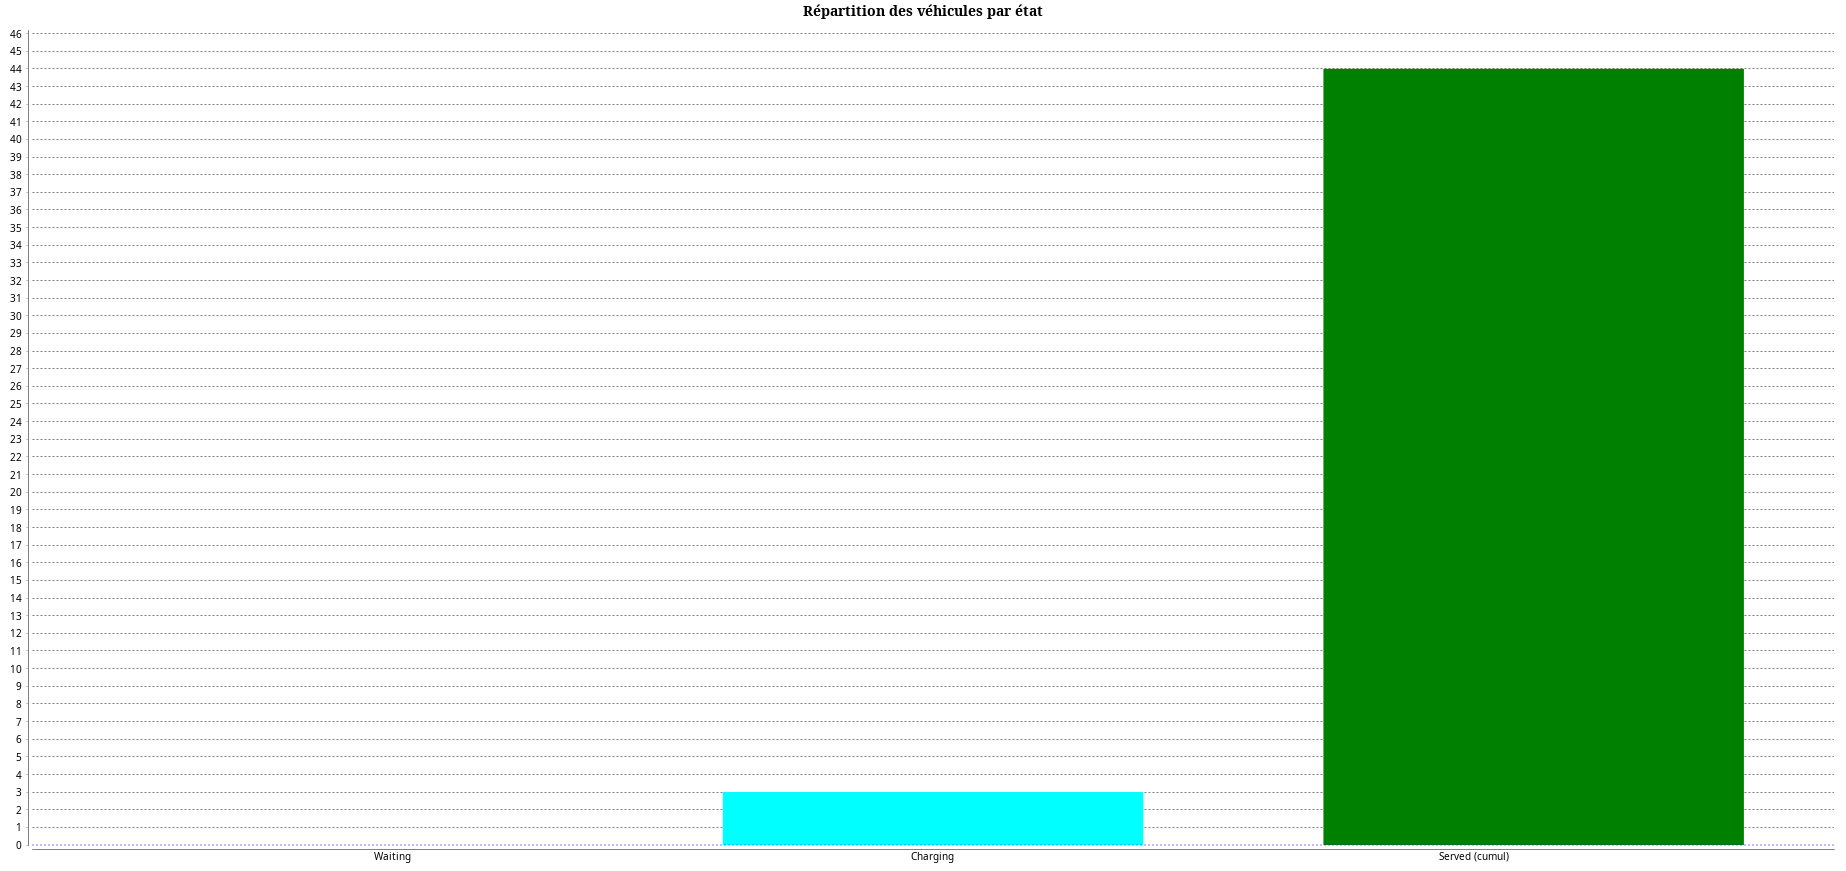
\includegraphics[width=0.82\textwidth]{ProjetSMA8_StationRecharge_model_display_Repartition_Vehicules_Hist_cycle_969_time_1778226082145.png}
\caption{Répartition des véhicules par état : en attente, en recharge et servis cumulés.}
\label{fig:repartition-vehicules}
\end{figure}

La Figure~\ref{fig:repartition-vehicules} résume l'état de la demande. Les véhicules en attente représentent la pression immédiate sur la station. Les véhicules en recharge occupent les ressources techniques. Les véhicules servis cumulés indiquent le débit déjà réalisé par le système. Ce graphique complète la carte spatiale en donnant une lecture quantitative des états des véhicules.

\begin{figure}[H]
\centering
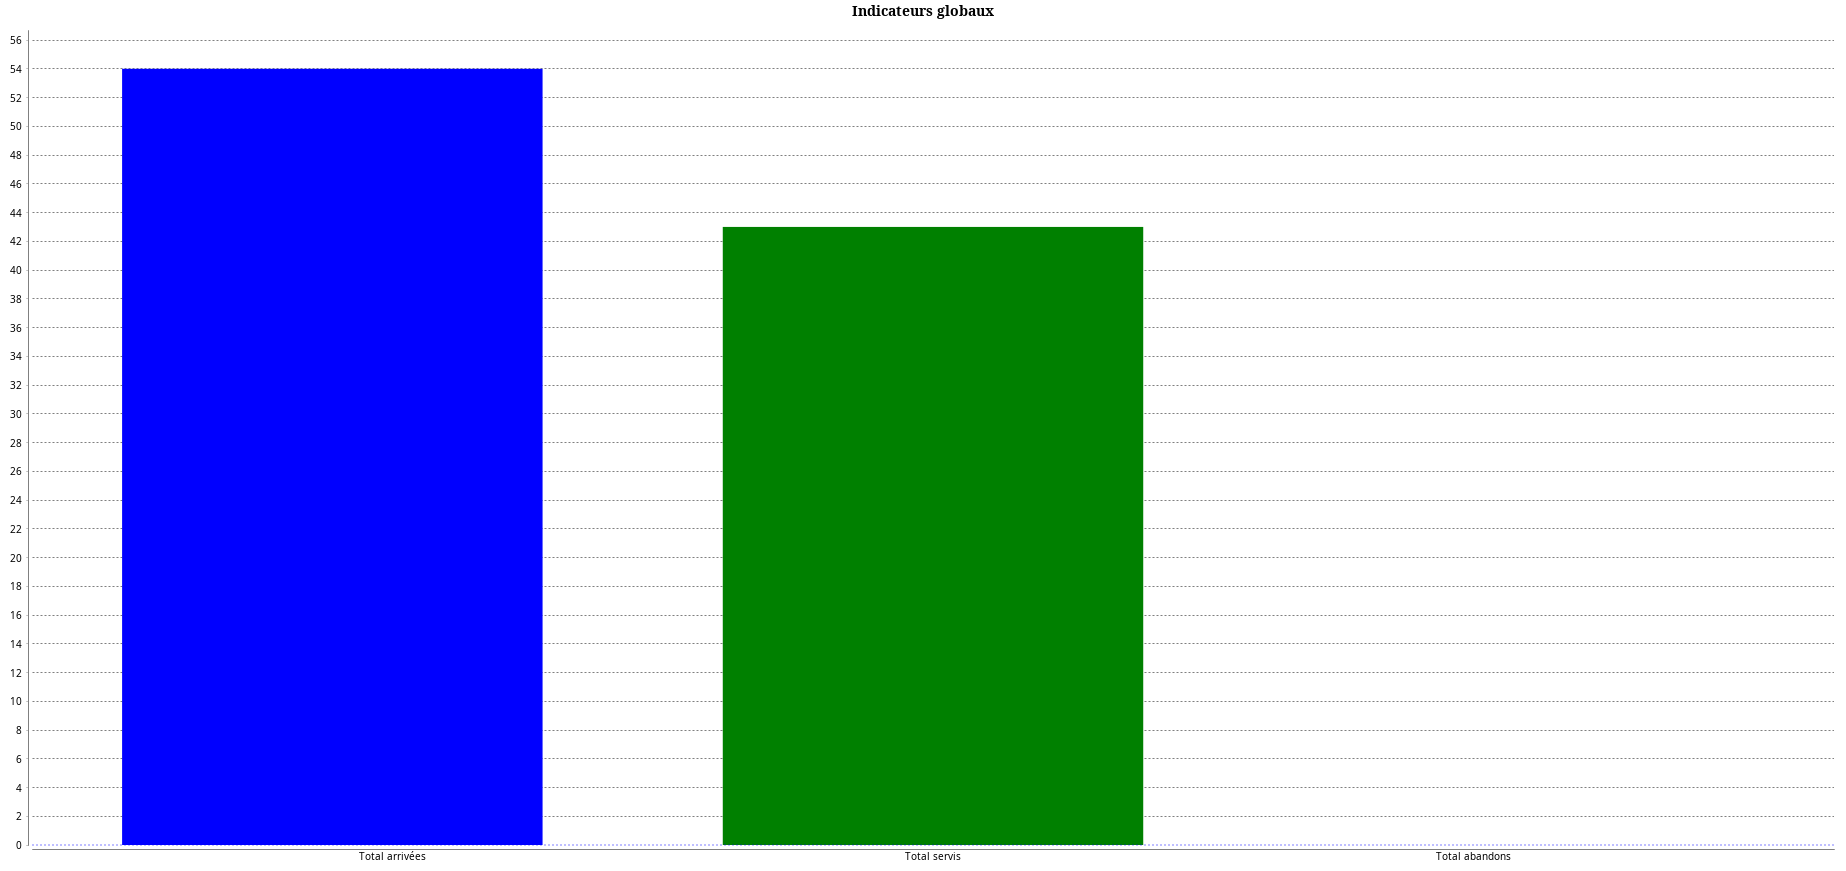
\includegraphics[width=0.82\textwidth]{ProjetSMA8_StationRecharge_model_display_Indicateurs_Globaux_Hist_cycle_969_time_1778226097003.png}
\caption{Indicateurs globaux cumulés : arrivées totales, véhicules servis et abandons.}
\label{fig:indicateurs}
\end{figure}

La Figure~\ref{fig:indicateurs} compare les flux cumulés du système. Les arrivées totales mesurent la demande reçue par la station. Les véhicules servis représentent la demande satisfaite. Les abandons signalent les véhicules qui n'ont pas obtenu de service dans des conditions acceptables. L'écart entre arrivées et véhicules servis s'interprète donc à la lumière des véhicules encore présents dans le système et des abandons déjà enregistrés.

\section{Conclusion}\label{sec:conclusion}

Ce travail a proposé une modélisation multi-agent d'une station de recharge pour véhicules électriques conformément au sujet 8. Le modèle représente explicitement les véhicules, les bornes et la station, ainsi que les principales interactions attendues : connexion directe, attente, sélection dans la file, recharge, abandon, panne et remise en file. La description par états discrets permet de suivre simultanément le parcours des véhicules et la disponibilité des bornes, tandis que la formulation mathématique précise les calculs déduits du code GAML.

La simulation met en évidence l'intérêt d'une approche multi-agent pour étudier un service soumis à une demande aléatoire et à des ressources limitées. Les indicateurs produits par GAMA permettent d'analyser l'occupation, la congestion, l'attente, l'abandon et la satisfaction. La configuration livrée dans ce rapport utilise 23 bornes, réparties en 10 lentes, 8 accélérées et 5 rapides. Cette capacité plus élevée doit réduire la pression sur la file par rapport à une station plus petite, mais la performance reste dépendante des arrivées groupées, des pannes et du facteur de puissance réseau.

La principale limite du modèle est que l'autre station mentionnée comme possibilité dans le sujet n'est pas explicitement représentée : un véhicule abandonné sort simplement du système. De plus, les préférences de puissance, l'urgence et la tolérance sont tirées aléatoirement et ne sont pas calibrées sur des données réelles. Les perspectives naturelles seraient d'exécuter plusieurs scénarios comparatifs en variant le nombre de bornes, la politique de file et l'information affichée, afin d'évaluer plus systématiquement la résilience de la station.

\newpage
\begin{thebibliography}{9}

\bibitem{kasereka_sma_2025}
Kasereka, S. (2025).
\emph{Système Multi-Agents}.
Notes de cours, Université de Kinshasa.

\bibitem{kasereka_gama_2025}
Kasereka, S. (2025).
\emph{Introduction à GAMA Platform}.
Support de travaux pratiques, Université de Kinshasa.

\bibitem{gama_charts}
GAMA Platform. (2026).
\emph{Defining Charts}.
\url{https://gama-platform.org/wiki/DefiningCharts}.

\bibitem{farkas2018}
Farkas, C., \& Telek, M. (2018).
Capacity Planning of Electric Car Charging Station Based on Discrete Time Observations and MAP(2)/G/c Queue.
\emph{Periodica Polytechnica Electrical Engineering and Computer Science}, 62(3), 82--89.
\url{https://doi.org/10.3311/PPee.11841}.

\bibitem{kim2017}
Kim, J., Son, S.-Y., Lee, J.-M., \& Ha, H.-T. (2017).
Scheduling and performance analysis under a stochastic model for electric vehicle charging stations.
\emph{Omega}, 66, 278--289.
\url{https://doi.org/10.1016/j.omega.2015.11.010}.

\bibitem{garcia2018}
García-Magariño, I., Palacios-Navarro, G., Lacuesta, R., \& Lloret, J. (2018).
ABSCEV: An agent-based simulation framework about smart transportation for reducing waiting times in charging electric vehicles.
\emph{Computer Networks}, 138, 119--135.
\url{https://doi.org/10.1016/j.comnet.2018.03.014}.

\bibitem{karlsson2023}
Karlsson, J., \& Grauers, A. (2023).
Agent-Based Investigation of Charger Queues and Utilization of Public Chargers for Electric Long-Haul Trucks.
\emph{Energies}, 16(12), 4704.
\url{https://doi.org/10.3390/en16124704}.

\bibitem{taillandier2019}
Taillandier, P., Gaudou, B., Grignard, A., Huynh, Q.-N., Marilleau, N., Caillou, P., Philippon, D., \& Drogoul, A. (2019).
Building, composing and experimenting complex spatial models with the GAMA platform.
\emph{GeoInformatica}, 23(2), 299--322.
\url{https://doi.org/10.1007/s10707-018-00339-6}.

\end{thebibliography}

\clearpage
\appendix
\section{Code GAML complet}\label{annexe:code}

Le code source est repris ci-dessous pour assurer la traçabilité entre la modélisation, les équations et les résultats.

\lstinputlisting{code/DUASENGE_MAYANO_PROJET8.gaml}

\end{document}
